\section{Euler's proof of the case \texorpdfstring{\(p = 2\), \(q = 3\)}{p = 2, q = 3}}

\begin{frame}
\frametitle{The case \texorpdfstring{\(p = 2\), \(q = 3\)}{p = 2, q = 3}}

\begin{theorem}[Euler, 1738]
The equation
\[
    x^2 - y^3 = 1
\]
has no solutions over \(\integers\) except for \(x = \pm 3\), \(y = 2\).
\end{theorem}

\vspace{1em}
\end{frame}

\begin{frame}
\frametitle{The case \texorpdfstring{\(p = 2\), \(q = 3\)}{p = 2, q = 3}}

In this case, the polynomial equation \(x^2 = y^3 + 1\) is an \textbf{elliptic curve}.

\begin{figure}
    \centering
    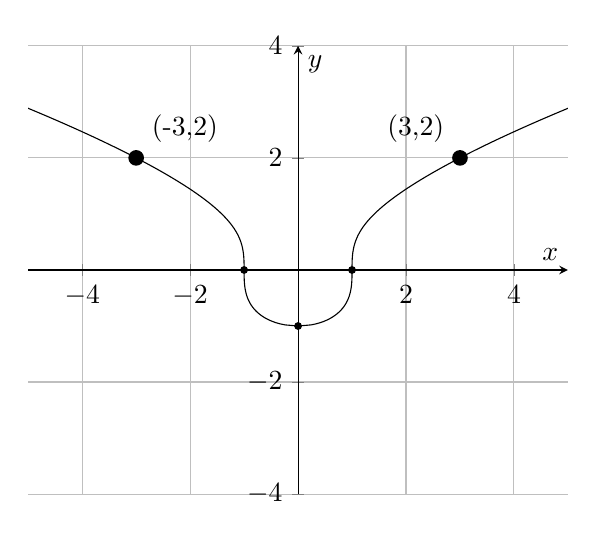
\begin{tikzpicture}
        \begin{axis}[
                axis x line=middle, axis y line=middle,
                xmin=-5,xmax=5, xlabel=$x$,
                ymin=-4,ymax=4, ylabel=$y$,
                grid=both,
            ]
            \addplot [domain=-1:3,samples=200]({sqrt(1 + x^3)},{x}); 
            \addplot [domain=-1:3,samples=200]({-sqrt(1 + x^3)},{x});

            \node[circle,fill,inner sep=1pt] at (axis cs:-1,0) {};
            \node[circle,fill,inner sep=1pt] at (axis cs:1,0) {};
            \node[circle,fill,inner sep=1pt] at (axis cs:0,-1) {};
            
            \node[label={45:{(-3,2)}},circle,fill,inner sep=2pt] at (axis cs:-3,2) {};
            \node[label={135:{(3,2)}},circle,fill,inner sep=2pt] at (axis cs:3,2) {};
        \end{axis}
    \end{tikzpicture}
\end{figure}
\end{frame}

\begin{frame}
\frametitle{The case \texorpdfstring{\(p = 2\), \(q = 3\)}{p = 2, q = 3}}

Switching \(x\) and \(y\), the polynomial becomes \(y^2 = x^3 + 1\). We can projectivize it by introducing a homogeneous coordinate \(z\):
\[
    E : y^2 z = x^3 + z^3
\]

\pause

Euler's theorem is implied by the following:
\begin{theorem}
The group \(E\left(\rationals\right)\) of rational points on the elliptic curve \(E\) is a cyclic group of order \(6\), consisting of
\[
    \Set{ \symcal{O}, (-1, 0), (0, 1), (0, -1), (2, 3), (2, -3) }
\]
where \(\symcal{O} = (0 : 1 : 0)\) is the point at infinity.
\end{theorem}
\end{frame}

\begin{frame}
\frametitle{Euler's proof of the case \texorpdfstring{\(p = 2\), \(q = 3\)}{p = 2, q = 3}}

Euler's proof \cite{Euler1914} relies on the method of \emph{descent}. Assuming the existence of a solution different from \((2, \pm 3)\), he obtains a new solution which is strictly ``smaller'' than the original solution.
\end{frame}

\begin{frame}
\frametitle{Euler's proof of the case \texorpdfstring{\(p = 2\), \(q = 3\)}{p = 2, q = 3}}

Suppose \(x^2 = y^3 + 1\). Write \(y = z - 1\). We have
\begin{gather*}
    x^2 = (z - 1)^3 + 1 = z^3 - 3 z^2 + 3 z - 1 + 1 \\
    \iff
    x^2 = z^3 - 3 z^2 + 3 z
\end{gather*}
Writing \(z = a/b\) for some \(a, b \in \integers^*\) with \(\gcd(a, b) = 1\), we get
\begin{gather*}
    x^2 = \left(\frac{a}{b}\right)^3 - 3 \left(\frac{a}{b}\right)^2 + 3 \frac{a}{b} \\[0.5em]
    \iff x^2 b^4 = a^3 b - 3 a^2 b^2 + 3 a b^3 \\[0.4em]
    \iff \left(x b^2\right)^2 = ab (a^2 - 3 a b + 3 b^2)
\end{gather*}
\end{frame}

\begin{frame}
\frametitle{Euler's proof of the case \texorpdfstring{\(p = 2\), \(q = 3\)}{p = 2, q = 3}}

Hence, we get that \(ab (a^2 - 3 a b + 3 b^2)\) is a square \(> 1\). The case \(a = 3\), \(b = 1\) is solution we know, so we may assume we have a different one. \\[1em]

Euler performs a series of substitutions and calculations to obtain a square of the same form, with
\[
    1 < u v (u^2 - 3 u v + 3 v^2) < ab(a^2 - 3ab + 3b^2)
\]
Repeating the process, we'd get an infinite descending chain of natural numbers, which is impossible.
\end{frame}

\begin{frame}
\frametitle{Generalizations}

Thinking about the second formulation of Euler's theorem, we see it's a result about points with rational coordinates on elliptic curves. \\[1em]

What can we say in general about the group of rational points of arbitrary elliptic curves?
\end{frame}

\begin{frame}
\frametitle{Generalizations: Mordell's Theorem}
\begin{theorem}[Mordell, 1922]
Let \(E\) be an elliptic curve with at least one rational point. Then \(E\left(\rationals\right)\) is a finitely-generated abelian group.    
\end{theorem}

\vspace{1em}

See \cite{Gondi2018_MordellTheorem} for an elementary proof.
\end{frame}

\begin{frame}
\frametitle{Generalizations: Mordell's Theorem}
In Euler's proof, we assumed the existence of a solution (different from the one we already knew) and reached a contradiction by constructing an infinite descending chain of ``smaller'' solutions. \\[1em]

Mordell proved his theorem in a similar way, starting with an arbitrary point on the curve and using descent to show that it must be generated by a set of points which are ``smaller''.
\end{frame}
